\section{Signalflussdiagram SFD}
\subsection{Definitionen}\script{54}
\begin{table}[H]
	\begin{tabular}{l|l}
		Knoten & Bestimmte Grössen (Variablen, Signale) \\
		Zweiz & Gewichtete Abhängigket \\
		Quelle & Knoten ohne einmündige Pfade \\
		Senke & Knoten ohne Ausgangs Pfade \\
		Gemischte Knoten & Knoten mit einmündung und Ausgang \\
		Pfade & eine Kontinuierliche Folge von Zweigen \\
		Schleife & Geschlossene Pfade (Ursprung und Endknoten sind dieselben)
	\end{tabular}
\end{table}

\subsection{Konstruktionsregeln}
\begin{enumerate}[nosep]
	\item Variablen stehen bei den Knoten, Konstanten oder Koeffisizen bei den Zweigen
	\item Signale durchlaufen Zweige in Pfeilrichtung
	\item Multiplikation eines Signales mit Pfeil-Transmittanz
	\item Variable ist die Summe der eingehenden Signale im Knoten
	\item Variable wird auf alle ausgehenden Zweige übertragen
\end{enumerate}
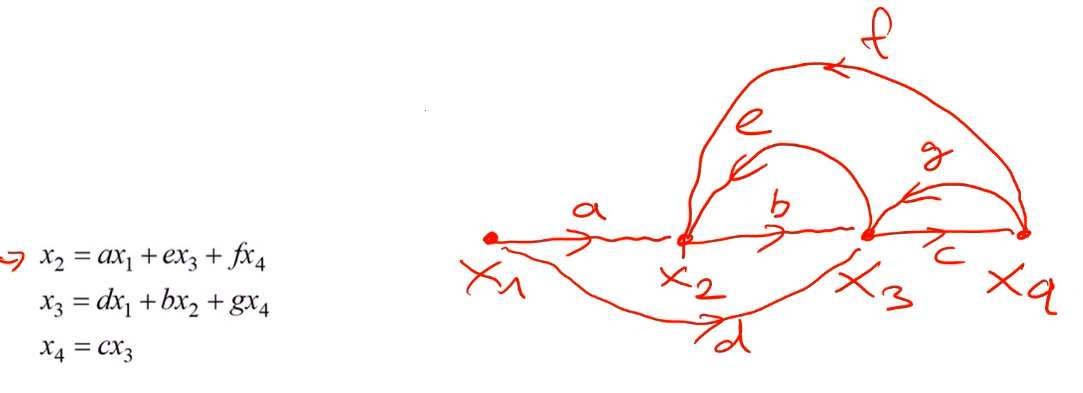
\includegraphics[width=\linewidth]{Images/sfd}

\subsection{Übertragungsfunktion}
Übertragungsfunktion UTF bestimmt die beziehung zwischem Ein- und Ausgangssignal eines Linearen Dynamischen Systems. UTF von $x_i$ nach $x_j$, wobei $x_i$ eine Quelle, $x_j$ jedoch nicht zwingend eine Senke sein muss wird im allgeminen folgendermassen definiert:
\[
H_{ij} = \frac{\sum_{k} P_{k}\cdot \Delta_k}{\Delta}
\]

\noindent$P_k$: \textbf{Vorwärtspfad} $k$ (start von Eingang): Multiplikation von jeder Sehne von Start bis Ziel\\
$\Delta_k$: \textbf{Kofaktor} des $k$-ten Pfades; 1 - (Summe aller Schleifen die $P_k$ nicht berühren) + (Summe aller Produkte zweier Schleifen, die $P_k$ und sich selbst nicht berühren) - (Summe aller Produkte dreier Schleifen, die $P_k$ und sich selbst nicht berühren) + $\dots$\\
$\Delta$: \textbf{Netzwerkdeterminante}; 1 - (Summe aller Schleifen) + (Summe aller Produkte zweier Schleifen, die sich nicht berühren) - (Summe aller Produktedreier Schleifen, die sich nicht berühren) + $\dots$\\

\noindent\textbf{Beispiel 1}:
SFD von folgender Schaltung:\\
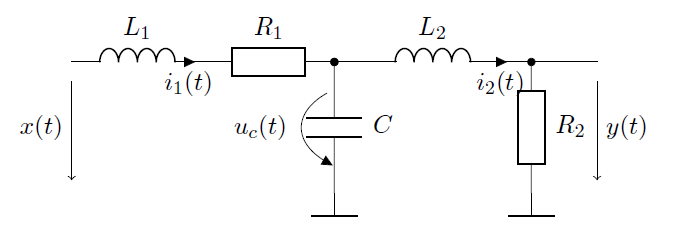
\includegraphics[width=\columnwidth]{Images/sfd_beispiel_adv}
Ergibt folgendes SFD\\
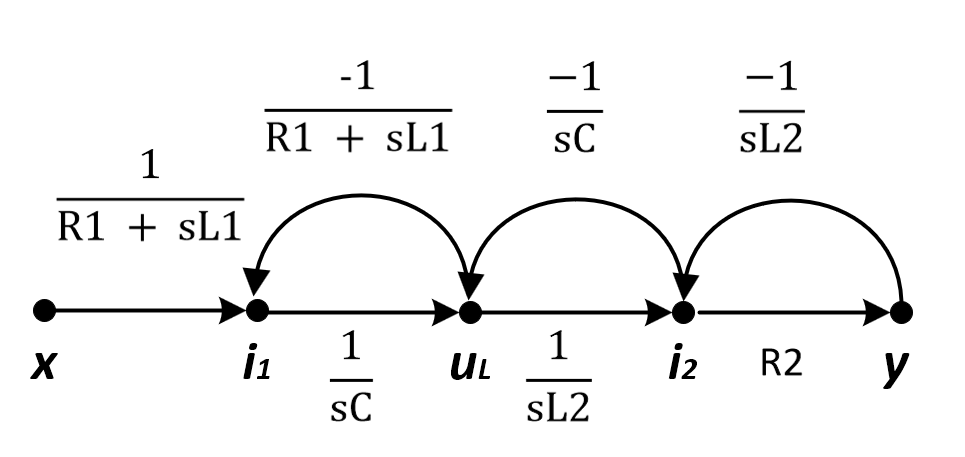
\includegraphics[width=\columnwidth]{Images/sfd_beispiel_adv1}
Darus kann nun die Übertragungsfunktion $H_{x,y}(s)$ berechnet werden
\begin{align*}
	H_{x,y}(s) &= \frac{\frac{1}{R_1+sL_1} \frac{1}{sC}\frac{1}{sL_2}R_2}{1-\left(\frac{-1}{R_1+sL_1}\frac{1}{sC}+\frac{-1}{sL_2}\frac{1}{sC}+\frac{-1}{sL_2}R2\right)+\frac{-1}{R_1+sL}\frac{1}{sC}\frac{-R_2}{sL_2}}
\end{align*}

\noindent\textbf{Hinweis für Elektro-Komponenten}
\begin{align*}
	\text{Kondensator}: \qquad U = \frac{1}{s C}I \\
	\text{Induktion}: \qquad U = s L I \\
\end{align*}

\noindent\textbf{Beispiel 2}: Es können für einfachere Netzwerke auch die Impedanzen berechnet werden und so die Übertragungsfunktion bestimmt werden:\\
\begin{center}
	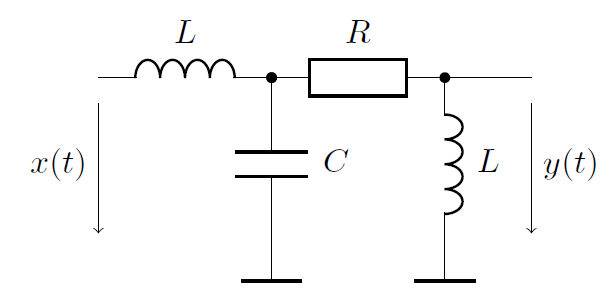
\includegraphics[width=0.8\columnwidth]{Images/sfd_beispiel_adv2}
\end{center}
\begin{align*}
	H(s) &= \frac{z}{sL + z} \cdot \frac{sL}{R + sL}  \qquad z = \frac{1}{sC + \frac{1}{r+ sL}}\\
	&= \frac{sL}{s^3L^2C + s^2RLC + s2L + R}
\end{align*}


\newpage
\subsection{Reduktionsregeln}
\noindent\textbf{Regel 1: Kettentransformation}\\
\script{59} Die gesamte übertragung einer Kaskade von Zweigen (d.h. einem Pfad) ist gleich dem Produkt der einzelnen Transmittanzen.\\
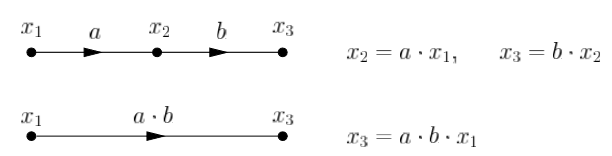
\includegraphics[width=\columnwidth]{Images/sfd_r1}~\\

\noindent\textbf{Regel 2: Paralleltransformation}\\
\script{59} Die gesamte Transmittanz paralleler Zweige ist gleich der Summe der einzelnen Zweigtransmittanzen.\\
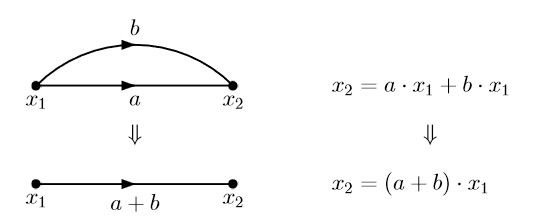
\includegraphics[width=\columnwidth]{Images/sfd_r2}~\\

\noindent\textbf{Regel 3: Enternung eines Knotens}\\
\script{60} Der Anfangs- oder Endpunkt einer Transmittanz kann entfernt
oder verschoben werden, solange die Transmittanz zwischen
den interessierenden Knoten im System unverändert bleibt.\\
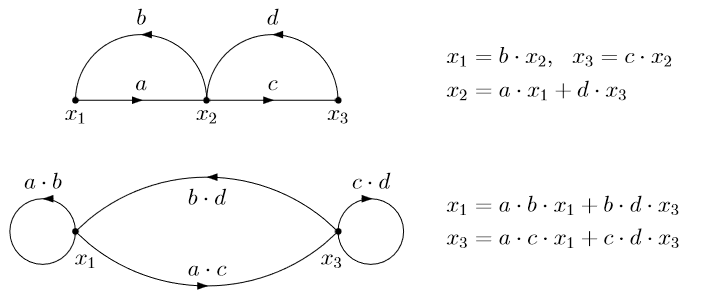
\includegraphics[width=\columnwidth]{Images/sfd_r3}~\\

\noindent\textbf{Regel 4: Transmittantverschiebung}\\
\script{60} Wichtig ist, dass eine neue Variable $x_3'$ eingeführt wird, wenn
der Endpunkt eines inneren Zweiges verschoben wird. (siehe c)\\
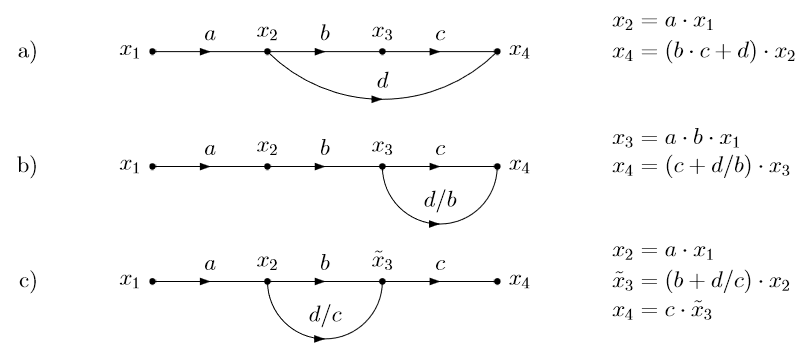
\includegraphics[width=\columnwidth]{Images/sfd_r4}~\\

\noindent\textbf{Regel 5: Pfadinversion}\\
\script{61} Es gilt zu beachten, das die Inversion eines Pfaden (dessen
Anfangspunkt nach Definition eine Quelle sein muss) den Effekt
hat, dass die Quelle vom einen Ende des Pfades zum
anderen Ende verschoben wird. Der Pfad von $x_i$ nach $x_j$ hat
eine Transmittanz von $L$. Den zu invertierenden Pfad setzten
wir $\frac{1}{L}$ und alle Pfade welche ursprünglich in $x_i$ endeten,
werden verschoben, dass sie neu in $x_j$ enden und ihre Transmittanzen
werden mit $-\frac{1}{L}$ multipliziert.\\
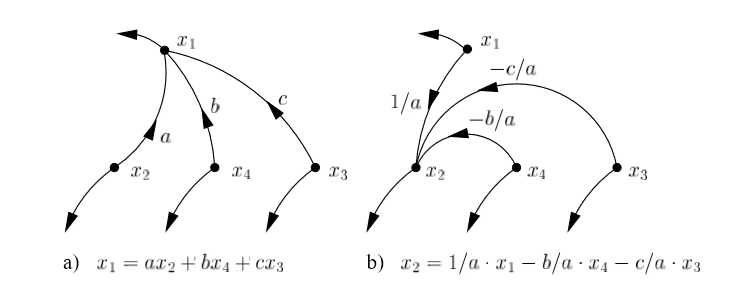
\includegraphics[width=\columnwidth]{Images/sfd_r5}~\\

\noindent\textbf{Regel 6: Entfernen einer Eigenschleife}\\
\script{62} Die Eigenschleife hat die Transmittanz $L$. Sie wird entfernt
indem man bei allen anderen Zweigen welche in den Knoten
münden, durch $(1 - L)$ dividiert.\\
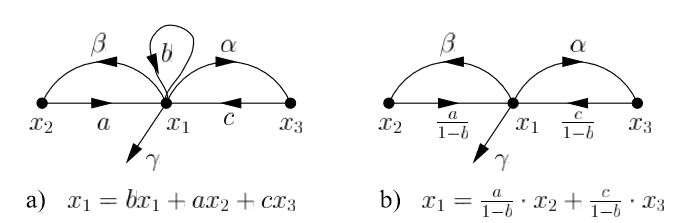
\includegraphics[width=\columnwidth]{Images/sfd_r6}~\\

\noindent\textbf{Regel 7: Schleifenreduktion}\\
\textbf{Einzel Schleife}\\
Die Transmittanz einer unabhängigen Variablen $x_i$ (d. h. einer
Quelle) zu einer abhängigen Variable (d. h. einem inneren
Knoten oder einer Senke) in einem SFD, das nur eine Schleife
und einen Vorwärtspfad enthält, ist gleich $Hij = \frac{P_{ij}}{1 - L}$ wobei
$P_{ij}$ die Transmittanz des Vorwärtspfades von $x_i$ nach $x_j$ und
$L$ die Transmittanz der Schleife ist. Die Formel lässt sich mittels
der Lösung des entsprechenden Gleichungssystems oder äquivalent 
durch Transmittanzverschiebung und Entfernung
der Eigenschleife beweisen.\\
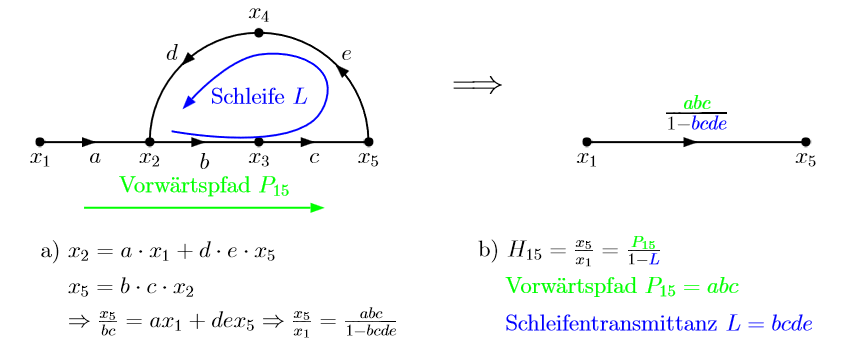
\includegraphics[width=\columnwidth]{Images/sfd_r7}~\\

\textbf{Mehrere sich nicht berührende Schleifen}\\
Bei einer Kaskade von sich nicht berührenden Schleifen (d.h.,
dass sie keine jeweils gemeinsamen Knoten haben) ist
die gesamte Transmittanz gleich dem Produkt der einzelnen
Transmittanzen: $H_{in} = \frac{P_{ij}}{1-L} \cdot \frac{P_{kj}}{1-L_k}\cdot \dots \cdot \frac{P_{(n-1)n}}{1-L_n}$\\
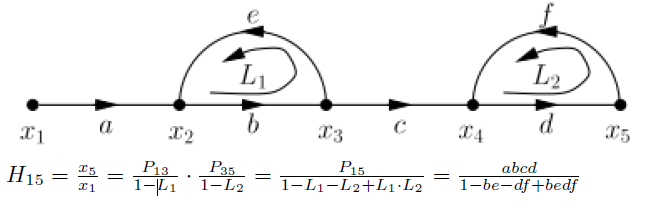
\includegraphics[width=\columnwidth]{Images/sfd_r7b}~\\

\textbf{Mehrere sich berührende Schleifen}\\
Für den Fall, dass die zwei Schleifen mindestens einen gemeinsamen
Knoten haben, ist die gesamte Transmittanz gegeben
durch: $H_{ij} = \frac{P_{ij}}{1 - L_i - Lj}$\\
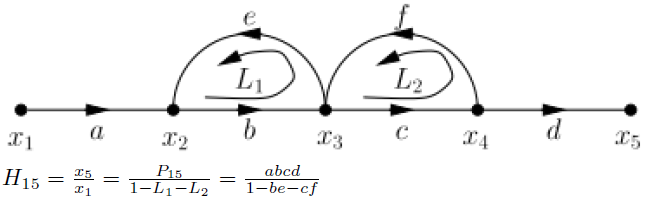
\includegraphics[width=\columnwidth]{Images/sfd_r7c}~\\


\noindent\textbf{Regel 8: Allgemeine Mehrfachschleifenreduktion}\\
\script{64} Wir betrachten hier den Mehrfachschleifenfall wo nur ein Pfad
zwischen einer Quelle $x_i$ und einem abhängigen Knoten $x_j$
existiert, wobei dieser Pfad jede Schleife im SFD berührt, (d.h. 
dass er wenigstens einen Knoten mit jeder Schleife gemeinsam
hat). Kurz ausgedrückt, lautet die Mehrfachschleifen Reduktionsregel für 
einfache Pfade: $H_{ij} = \frac{P_{ij}}{\Delta}$
Die Grösse $\Delta$ ist die Graph oder Netzwerkdeterminate und wird folgendermassen ermittelt:~\\
$\Delta$  = 1 - (Summe alle Schleifen) + (Summe aller Produkte zweier Schleifen, die sich nicht berühren) - (Summe aller Produkte dreier Schleifen, die sich nicht berühren) + $\dots$
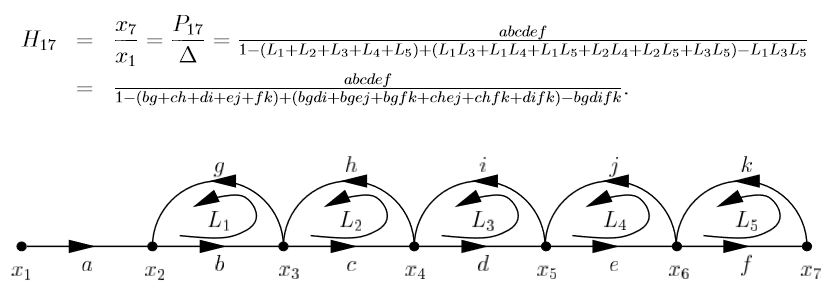
\includegraphics[width=\columnwidth]{Images/sfd_r8}~\\

\textbf{Regel 9: Mason's Regel}\\
UTF von $x_i$ nach $x_j$ , wobei $x_i$ eine Quelle, $x_j$ jedoch nicht zwingend eine Senke sein muss.
\[
H_{ij} = \frac{\sum_{k}P_k\cdot\Delta_k}{\Delta}
\]
$P_k \Rightarrow$ Vorwärtspfad $k$ (bezogen auf 1 Eingang)\\
$\Delta_k \Rightarrow $ 1 - (Summe alle Schleifen die $P_k$ nicht berühren) + (Summe aller Produkte zweier Schleifen, die $P_k$ und sich selbst nicht berührenn) - (Summe aller Produkte dreier Schleifen, die $P_k$ und sich selbst nicht berührenn) + $\dots$\\
$\Delta \Rightarrow $ 1 - (Summe alle Schleifen) + (Summe aller Produkte zweier Schleifen, die sich nicht berühren) - (Summe aller Produkte dreier Schleifen, die sich nicht berühren) + $\dots$\\
~\\ \textbf{Beispiel}\\
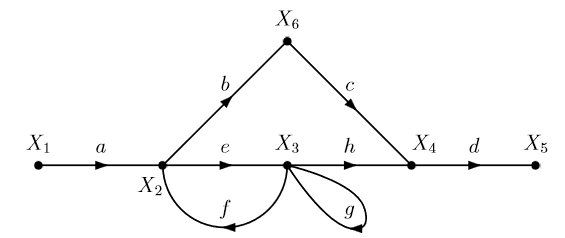
\includegraphics[width=\columnwidth]{Images/sfd_beispiel}
Die UTF zwischen $x_1$ und $x_4$ ist mit Mason's Regel:
\[
H_{1,4} = \frac{x_4}{x_1} = \frac{aeh \cdot 1 + abc - abcg}{1 - ef - g}
\]

\subsection{Ordnung}
Die Ordnung kann durch die Anzahl der aufgetrennten Knoten bestimmen werden, bis SFD schleifenfrei ist.\\
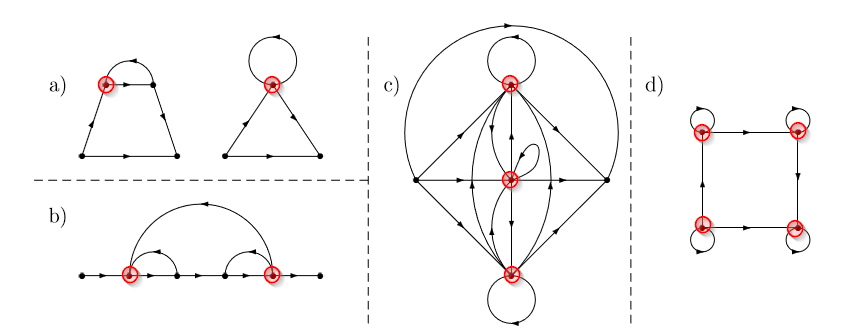
\includegraphics[width=\columnwidth]{Images/sfd_ordnung}


\subsection{SFD von Operationsverstärker}
\includegraphics[width=\columnwidth]{"./Images/sfd_op"}
